\documentclass{beamer}

\usetheme{Goettingen}

\usepackage[french]{babel}
\usepackage[utf8]{inputenc}
\usepackage[T1]{fontenc}
\usepackage{lmodern}
\usepackage{graphicx}
\usepackage{color}
\usepackage{amsmath, amssymb}
\newcommand{\R}{\mathbb{R}}
\newcommand{\Z}{\mathbb{Z}}

\author{Gaspard Jankowiak \quad Antoine Levitt\\ Tuteur : Antoine Girard}
\title{{\textbf{\textcolor{black}{Projet Spécialité Ensimag 2A}}}\vspace{1cm}\\ {Ajustement d'opinions et création de communautés dans des réseaux
sociaux}}
\date{19 juin 2009}

\begin{document}
\begin{frame}
	\maketitle
\end{frame}

\begin{frame}{Contexte}
  \begin{itemize}
  \item Graphe non orienté connexe $(V, E)$.
  \item $N_i = \{j\, |\, \{i, j\} \in E\}$ voisinage du noeud $i$.
  \item Chaque noeud $i$ est un agent avec une opinion $x_i \in
    \mathbb {R}$.
  \item Evolution de cette opinion $x_i$ selon un modèle.
  \item Dynamique utile pour comprendre le graphe.
  \end{itemize}
\end{frame}

\begin{frame}{Analyse matricielle de graphes}{Définitions}
  \begin{itemize}
  \item Degré d'un noeud $d_i$.
  \item Matrice des degrés $D$ : $D_{i i} = d_i$.
  \item Matrice d'adjacence $A$ : $A_{i j} = 1$ si $\{i,j\} \in E$,
    $0$ sinon.
  \item Matrice Laplacienne $L = D - A$.
  \item $(L x)_i = d_i x_i - \sum_{j \in N_i} x_j$.
  \item Analogue pour les graphes du Laplacien discret $\Delta$, au signe près.
  \end{itemize}
\end{frame}

\begin{frame}{Evolution des opinions}{Modèle continu}
  \begin{itemize}
  \item   $\dot{x} + L x = 0$
  \item ``Équation de la chaleur'' pour un graphe.
  \item $\dot{x}_i = \sum_{j \in N_i} (x_j - x_i)$.
  \item Modification de l'opinion de chaque agent en fonction des voisin.
  \item Vecteur propre de $L$ $(1, 1, \dots, 1)^T$ associé à $0$ :
    conservation de la moyenne.
  \item $L$ symétrique positive, $\lambda_1 = 0 < \lambda_1 \leq
    \lambda_2 \leq \dots \leq \lambda_n$.
  \item Convergence vers la valeur moyenne selon $x(t) - x_\text{moy}
    \approx K v_2 e^{-\lambda_2 t}$.
  \item $\lambda_2$ est la {\bf connectivité algébrique} du graphe.
  \end{itemize}
\end{frame}

\begin{frame}{Evolution des opinions}{Modèle discret}
  \begin{itemize}
  \item Dur à simuler et modifier : passage au discret.
  \item Méthode d'Euler : $x(t+1) = (I - \alpha L) x(t)$ pour $\alpha$
    petit.
  \item $x_i(t+1) = x_i(t) + \alpha \sum_{j \in N_i} (x_j(t) - x_i(t))$
  \item Même analyse, $x(t) - x_\text{moy} = K v_2 (1 - \alpha
    \lambda_2)^t$.
  \item $\alpha$ fixé suffisamment petit pour éviter les instabilités.
  \item Modèle utilisé en pratique.
  \item Plus facile à modifier.
  \end{itemize}
\end{frame}

\begin{frame}{Evolution}{Forçage}
  \begin{itemize}
  \item Forcer la convergence du système.
  \item $N'_{i}(t) = \{j \in N_i, ||x_i(t) - x_j(t)|| < R \rho^t\}.$
  \item Restriction du graphe de communication : convergence plus rapide.
  \item Si la convergence n'est pas assez rapide, on abandonne le
    consensus : coupures et formation de communautés.
  \item On attend une bifurcation pour $\rho = \lambda_2$.
  \item Les communautés sont-elles intrinsèques au graphe ?
  \item Étude numérique.
  \end{itemize}
\end{frame}

\begin{frame}{Graphes utilisés}{Graphes réels}
	\begin{center}
		\begin{tabular}[h]{cc}
			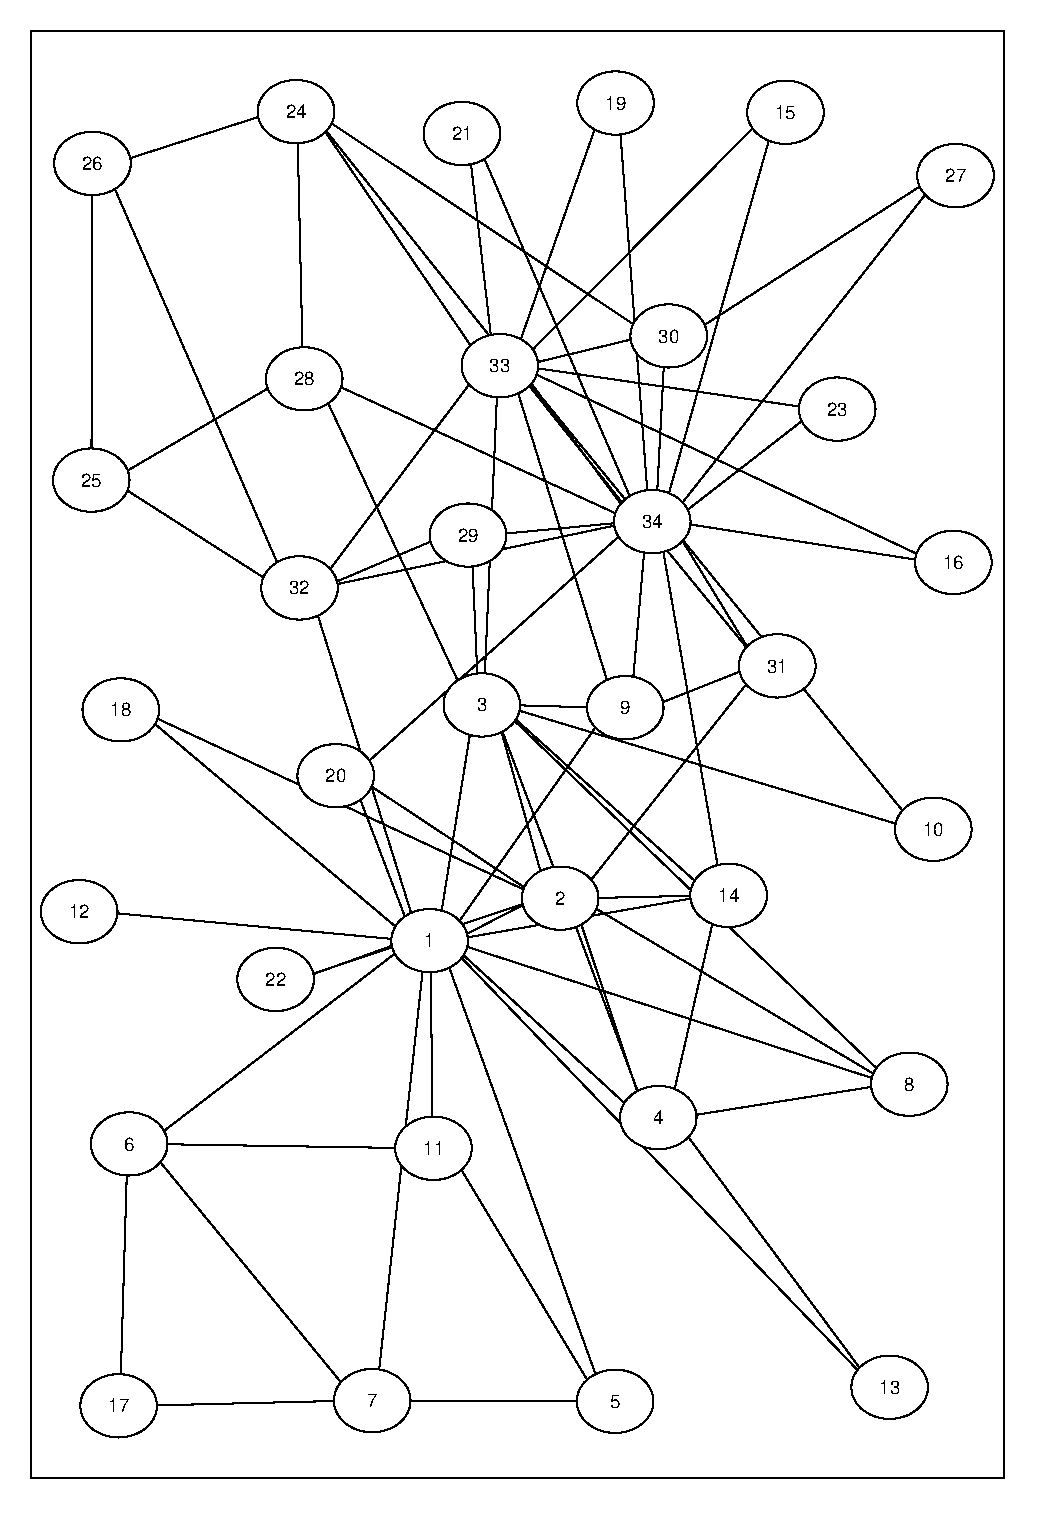
\includegraphics[width=0.4\textwidth]{pres-za}&
			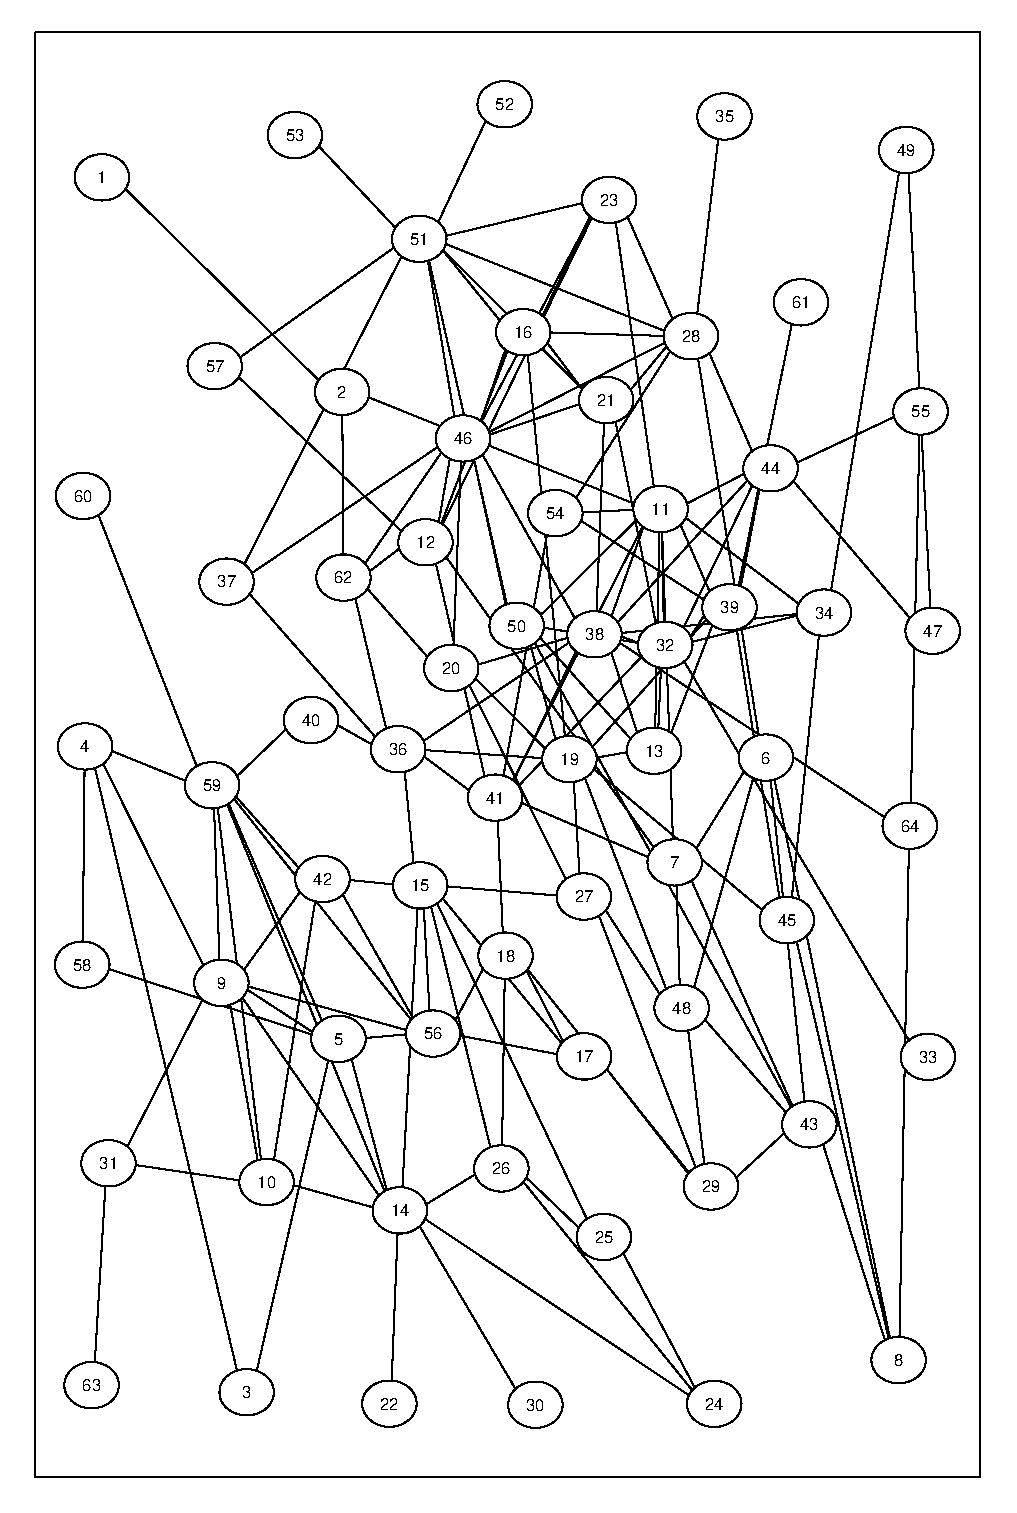
\includegraphics[width=0.4\textwidth]{pres-do}
			\\
			Club de karaté Zachary & Banc de dauphins
		\end{tabular}
	\end{center}
\end{frame}

\begin{frame}{Evolution temporelle}{Consensus : $\rho > \lambda_2$} 
	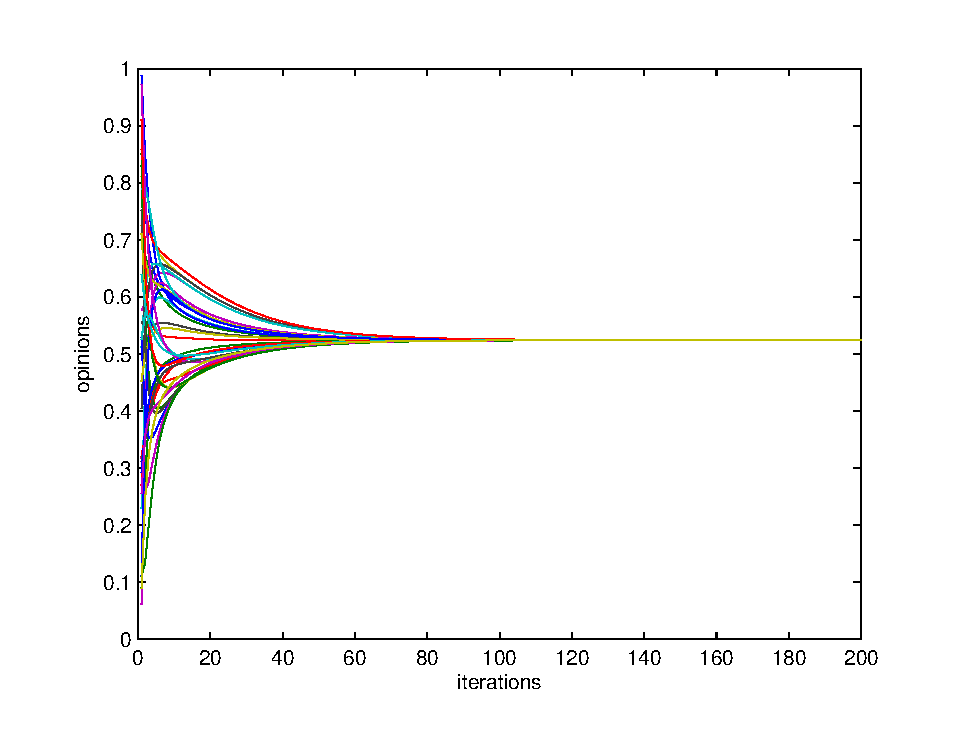
\includegraphics[width=\textwidth]{evolution_ok}
\end{frame}
\begin{frame}{Evolution temporelle}{Apparition de groupes : $\rho < \lambda_2$}
	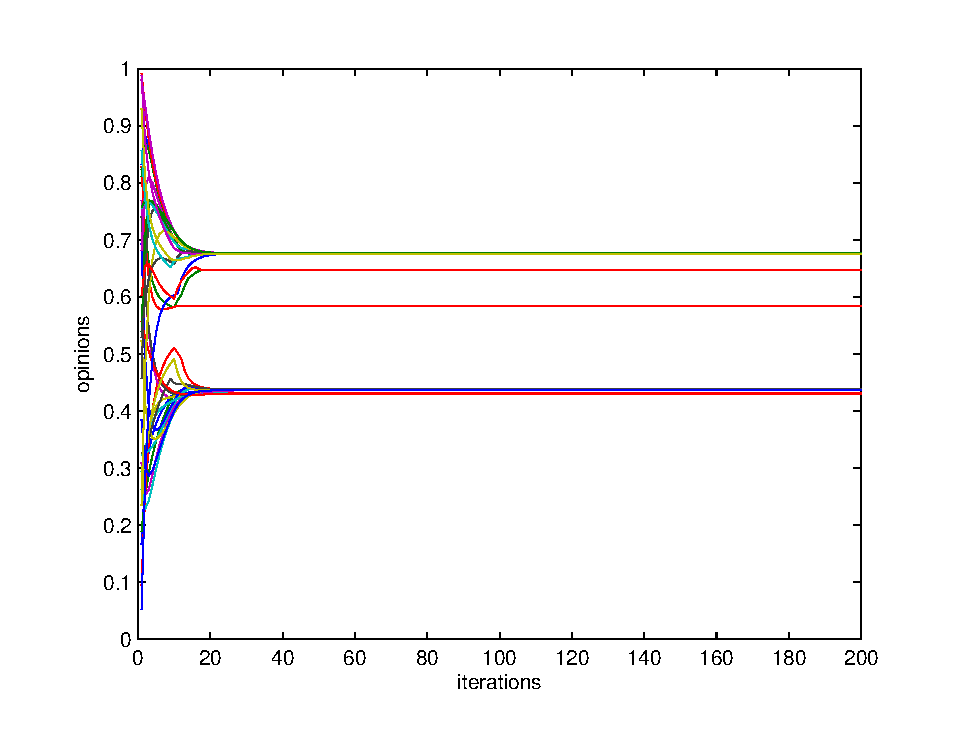
\includegraphics[width=\textwidth]{evolution_clusters}
\end{frame}

\begin{frame}{Détection des groupes}
	Groupes $\equiv$ composantes connexes du graphe :
	$$N'(t)=\bigcup_i N'_i(t).$$

	Rappel : $N'_i(t) = \{j \in N_i, ||x_i - x_j|| < R \rho^t\}.$
\end{frame}

\begin{frame}{Formation de groupes}
	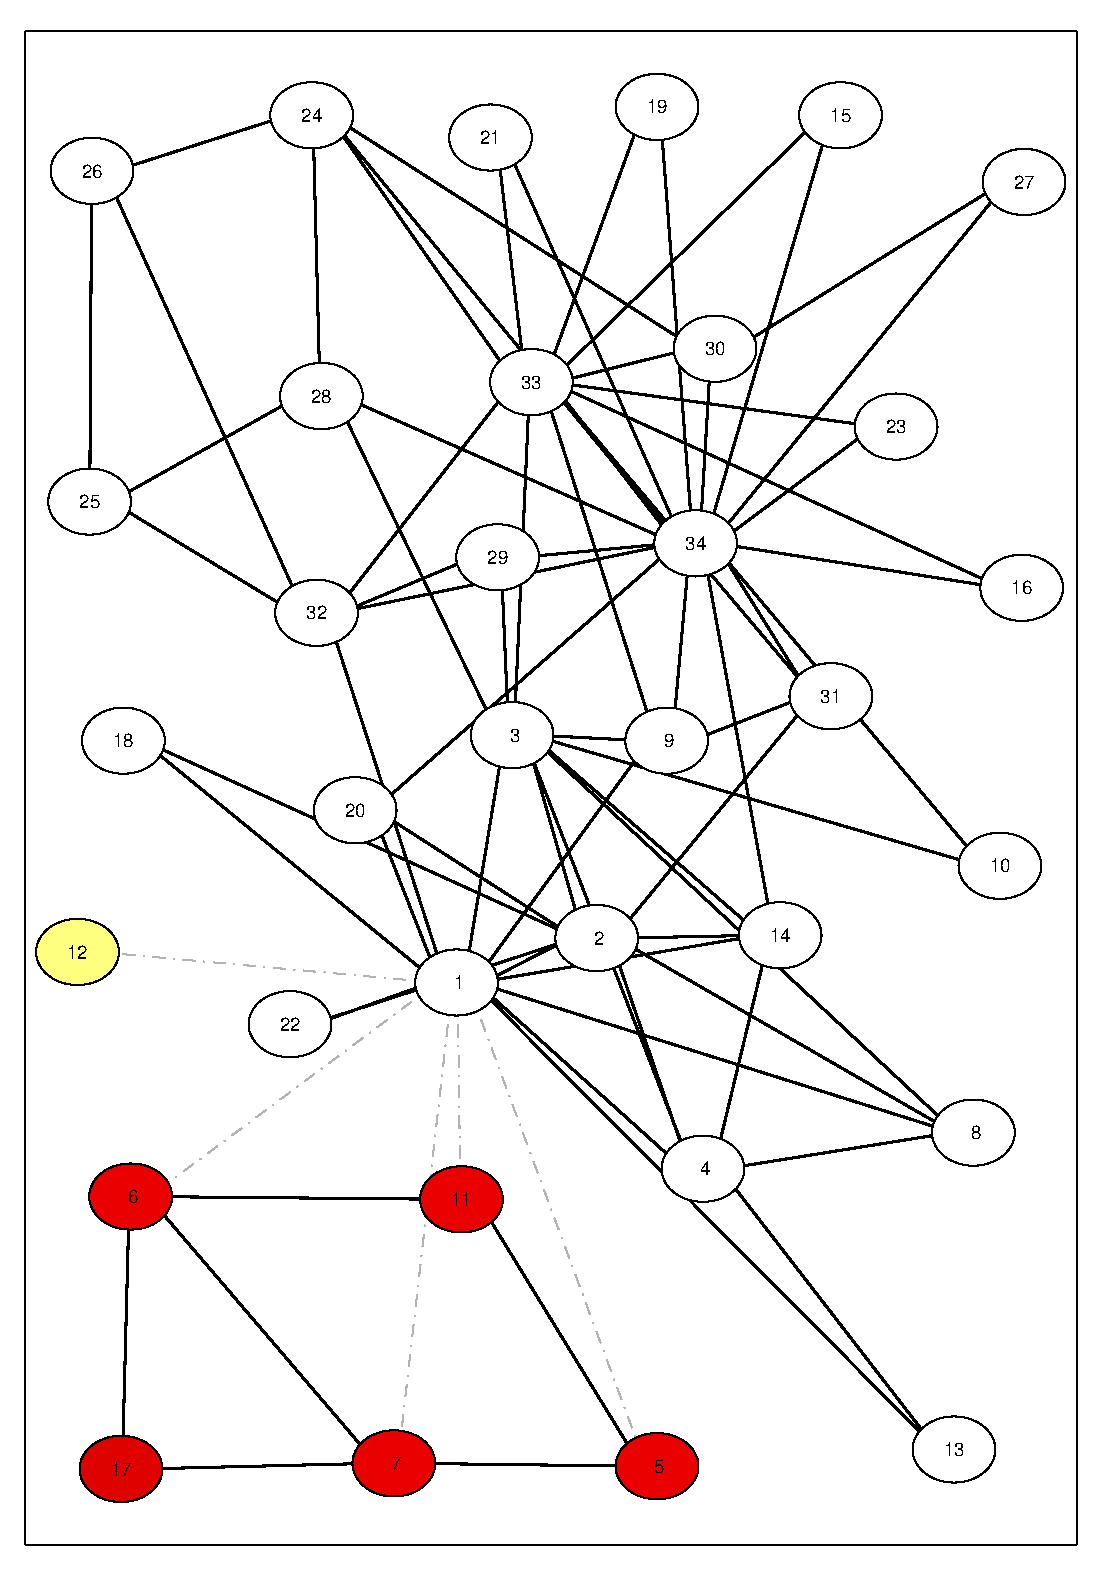
\includegraphics[width=.5\textwidth]{za-m1-3}
	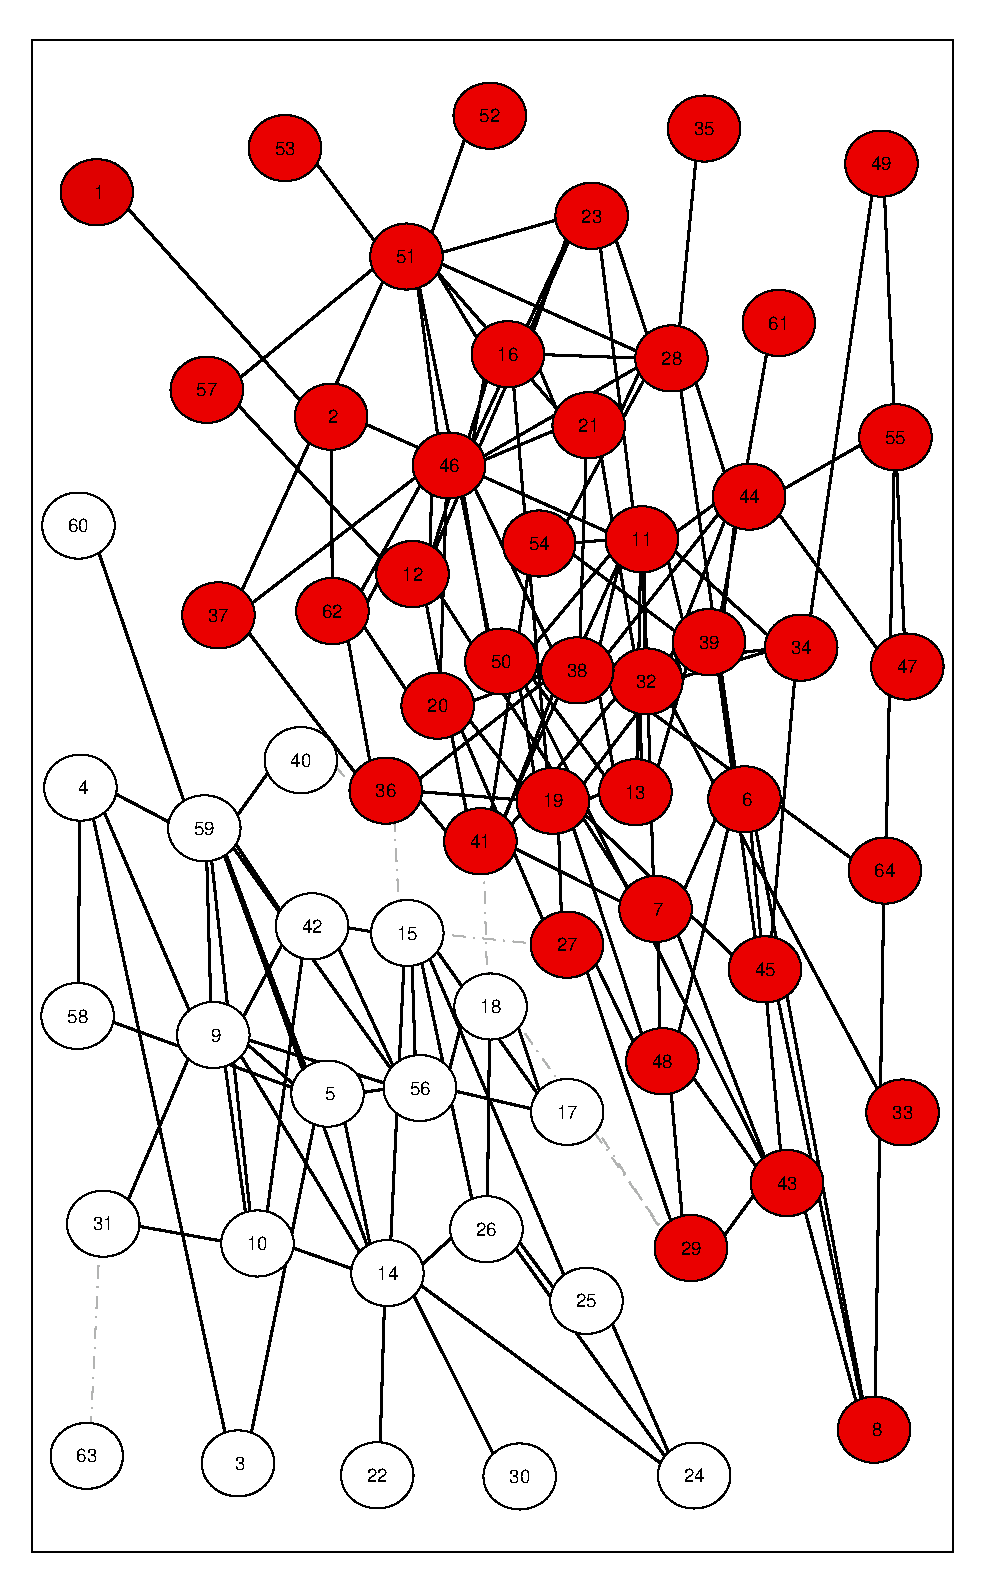
\includegraphics[width=.5\textwidth]{do-m1-3}
\end{frame}

\begin{frame}{Bifurcation pour $\rho = \lambda_2$}{Graphe club de karaté de Zachary, $\rho = 0,953$}
	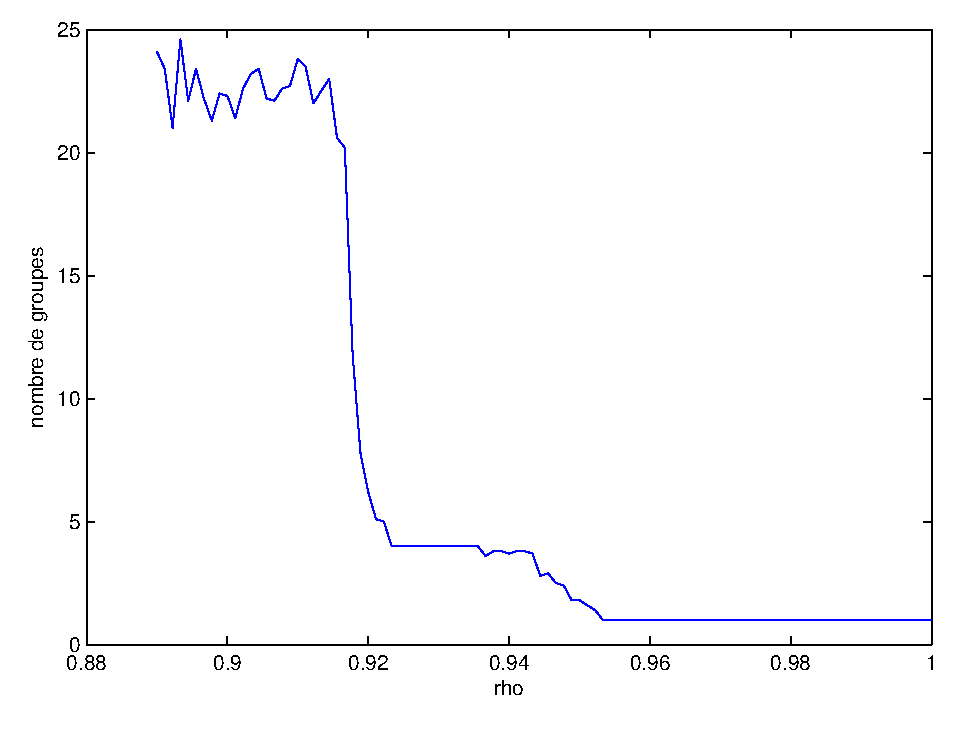
\includegraphics[width=\textwidth]{bifur}
\end{frame}

\begin{frame}{Problèmes numériques}
	\begin{center}
		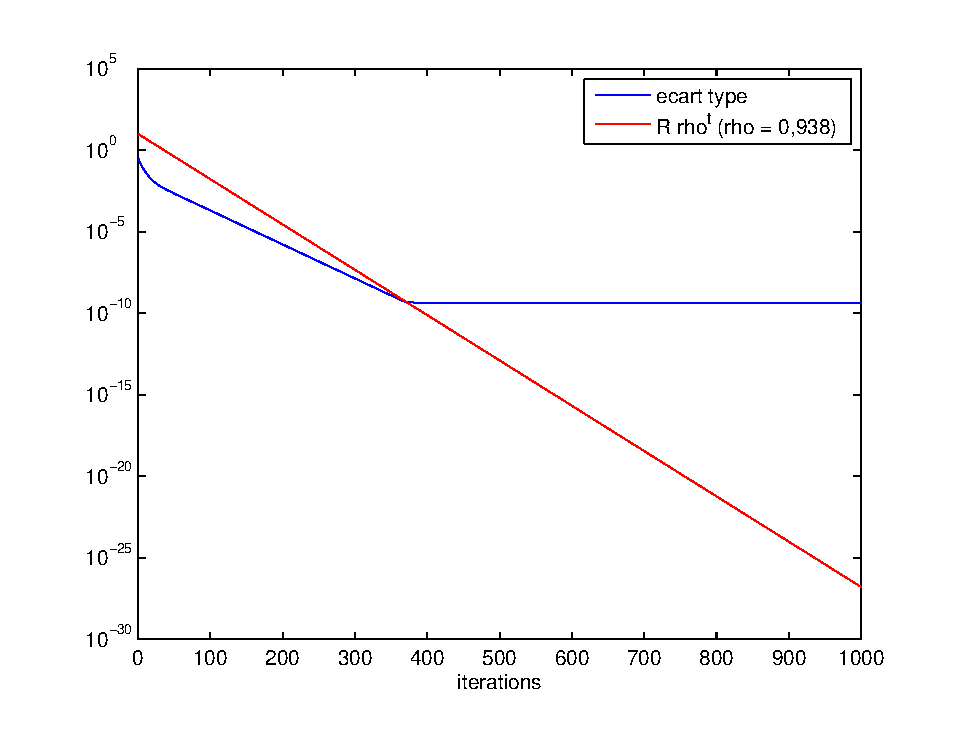
\includegraphics[width=.4\textwidth]{var_rho_0938}
		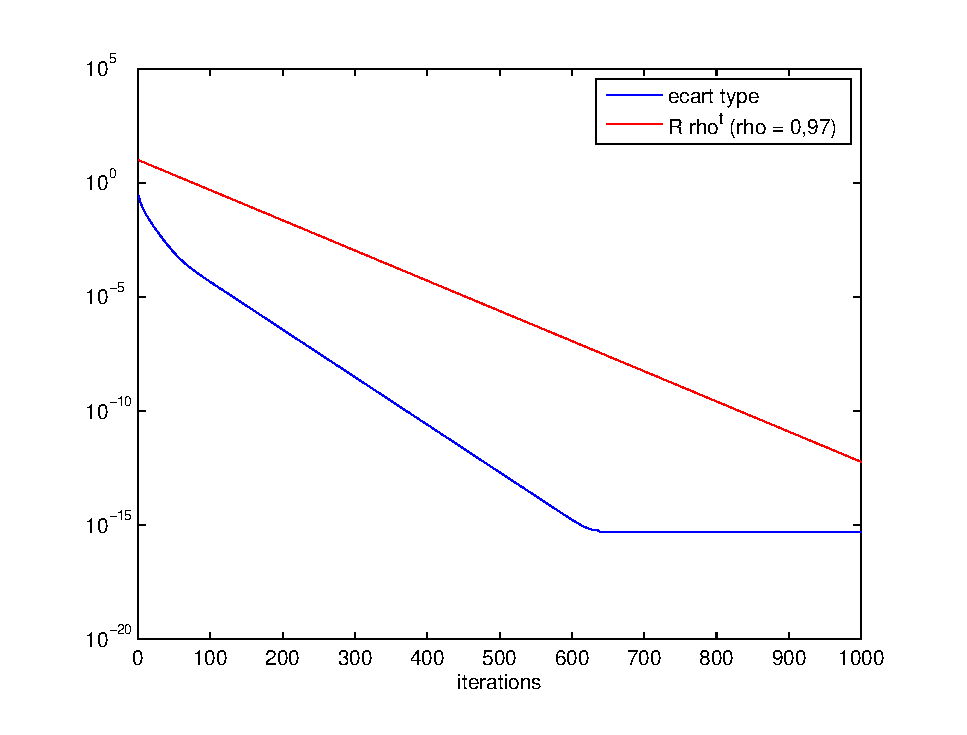
\includegraphics[width=.4\textwidth]{var_rho_097}\\
		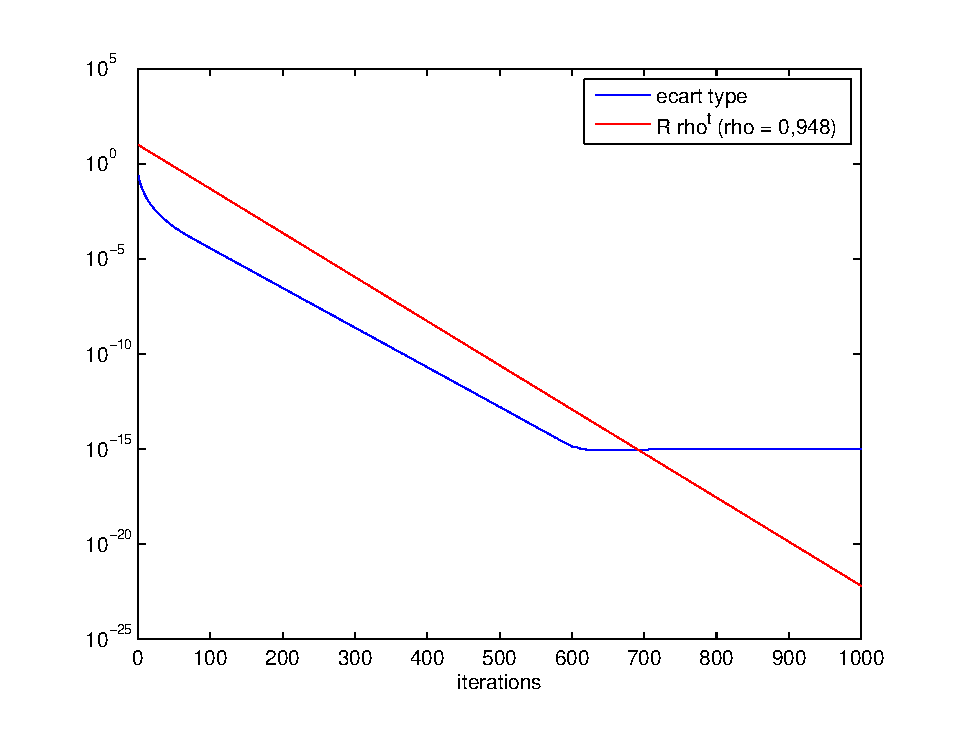
\includegraphics[width=.6\textwidth]{var_rho_0948}
	\end{center}
\end{frame}

\begin{frame}{Partitionnement spectral}
  blah
\end{frame}

\begin{frame}{Résultats}{Spectres}
		\begin{center}
			Spectres des Laplaciennes des deux graphes étudiés :
			\begin{description}
				\item[\alert{Rouge}] : Dauphins
				\item[Bleu] : Zachary
			\end{description}
			\bigskip
			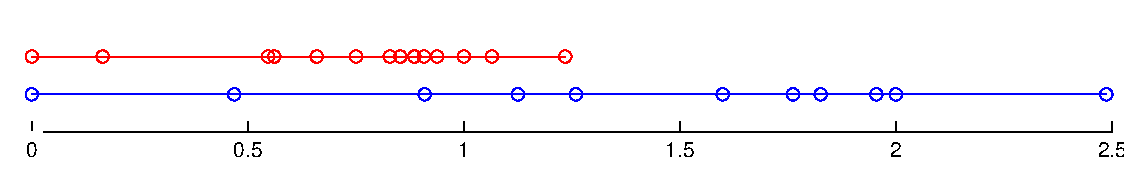
\includegraphics[width=\textwidth]{new_plots/spectres}\\
			\bigskip
			Deux méthodes pour la division spectrale :
			\begin{enumerate}
				\item Grouper les n\oe uds ayant une composante positive sur $v$, et ceux ayant une composante négative.
				\item Trier les n\oe uds selon leur composantes sur $v$ et couper au plus grand écart.
			\end{enumerate}
		\end{center}
\end{frame}

\begin{frame}{Résultats}{Zachary}
	\begin{center}
		\begin{tabular}[h]{ccc}
		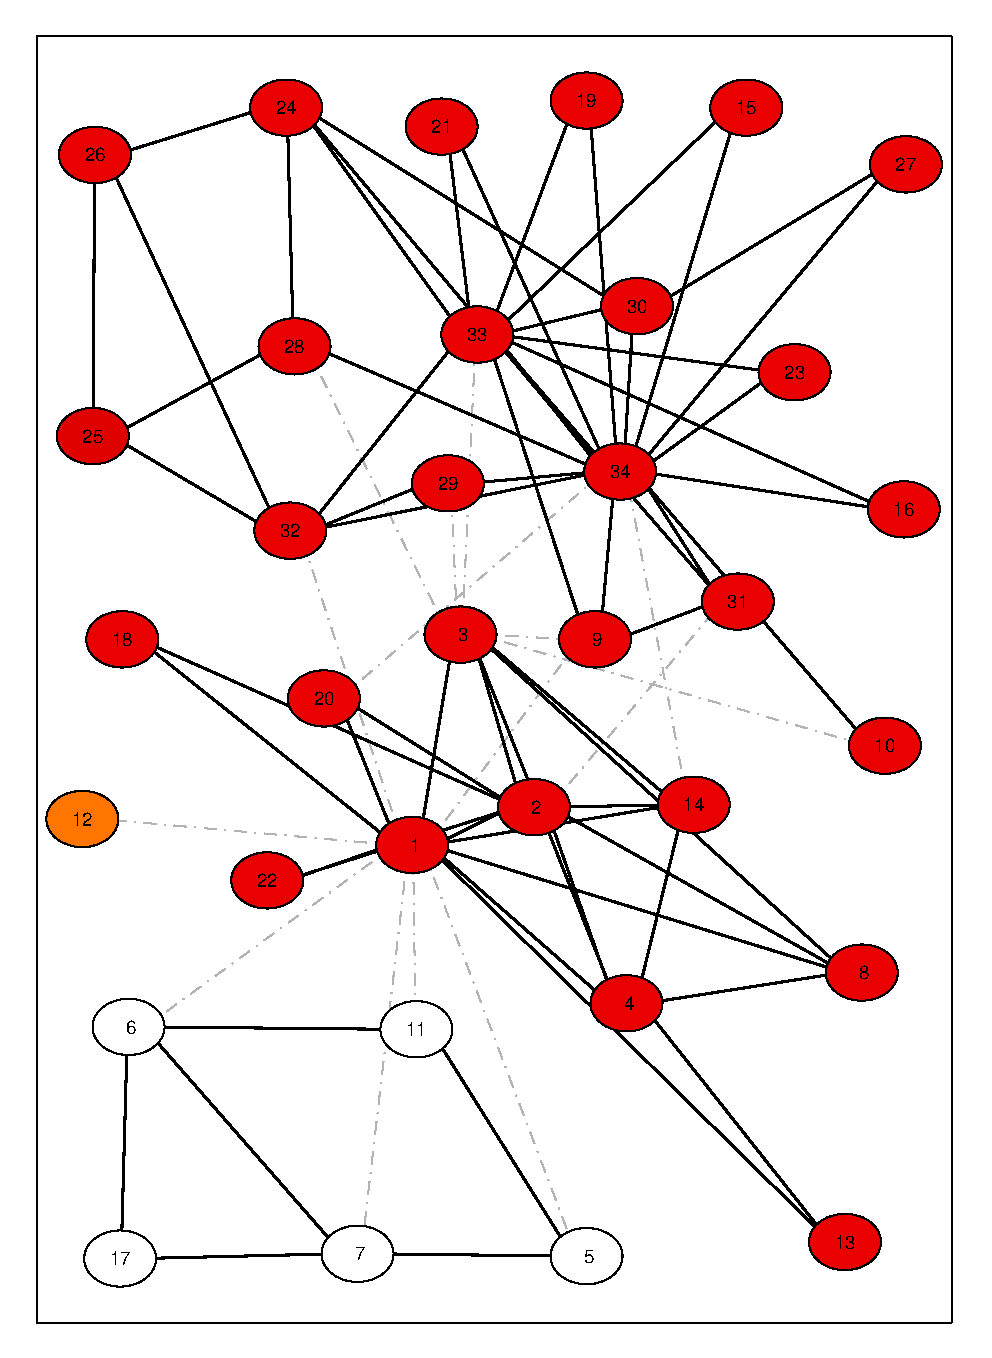
\includegraphics[width=0.30\textwidth]{new_plots/za-m1}&
		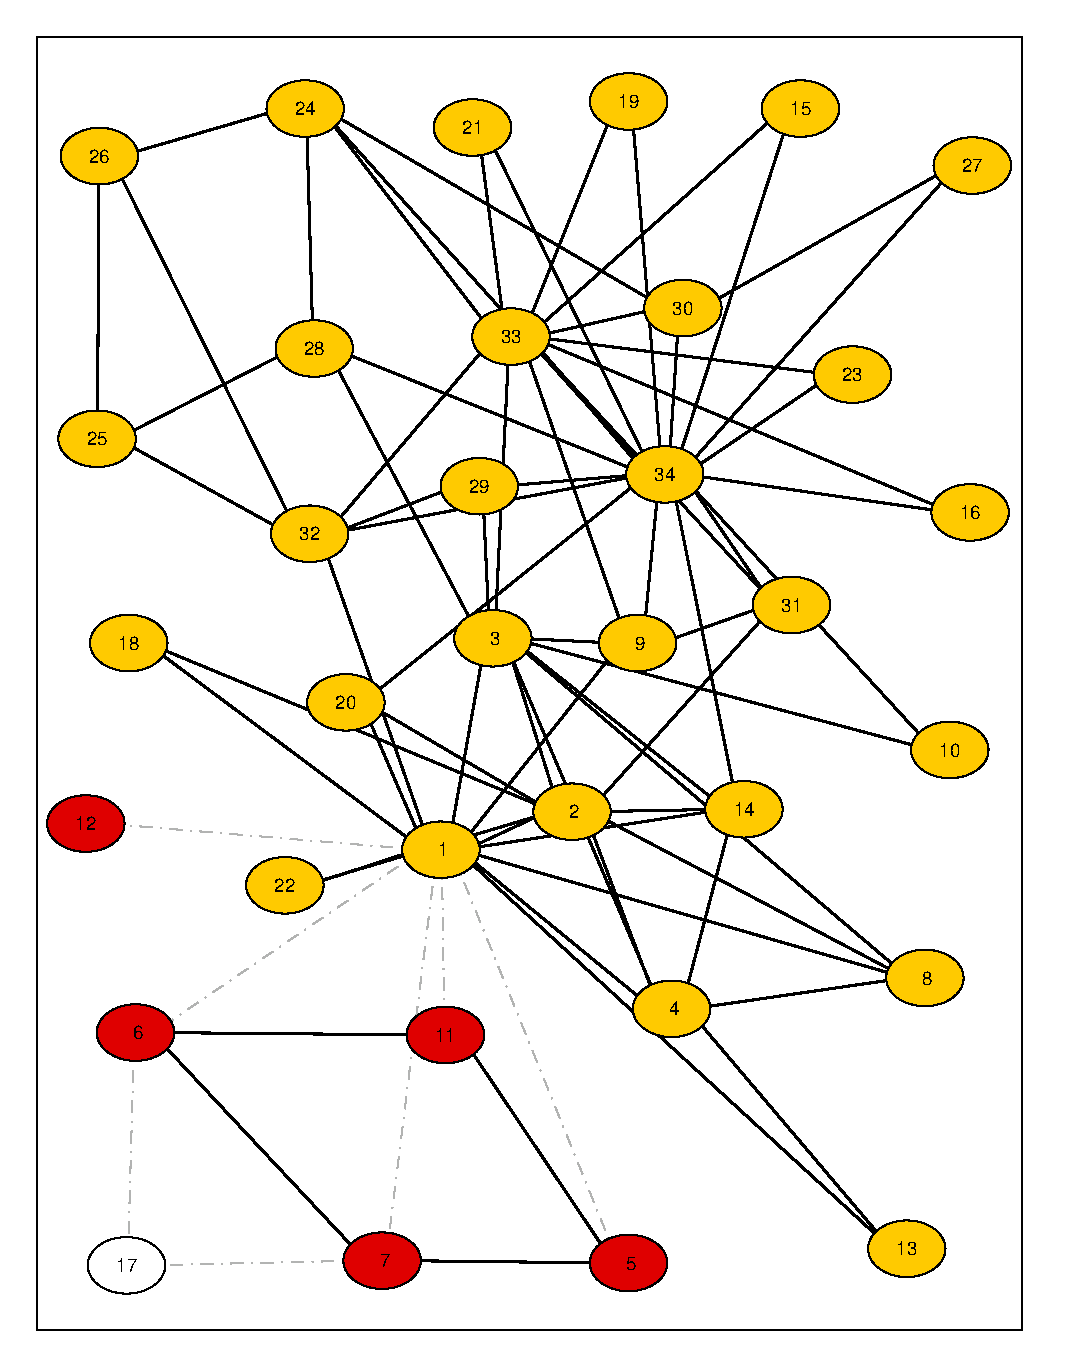
\includegraphics[width=0.30\textwidth]{new_plots/za-sp-ge}&
		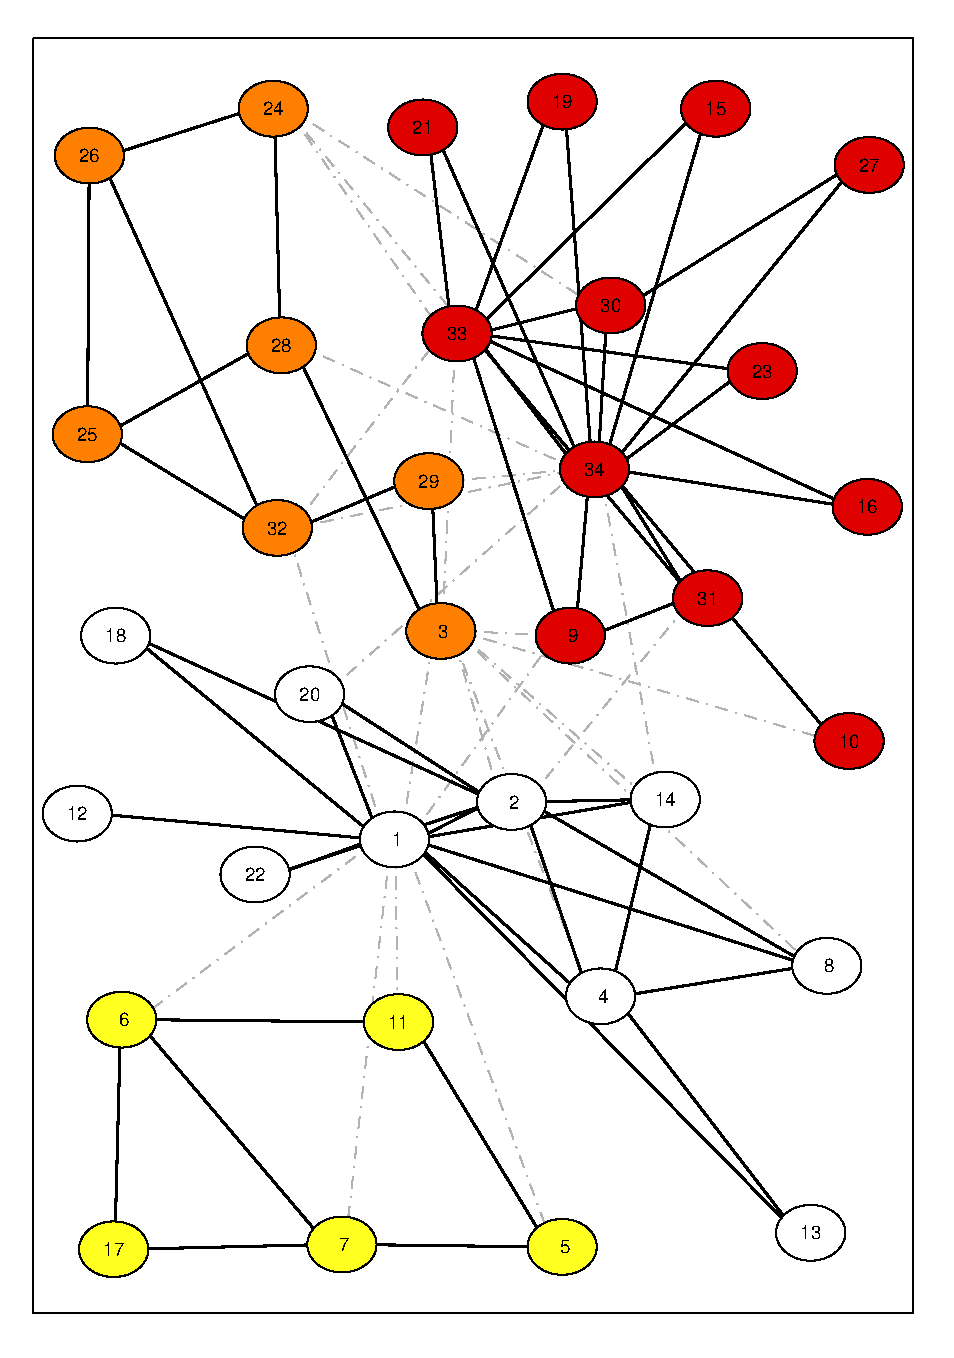
\includegraphics[width=0.30\textwidth]{new_plots/za-m2}
		\\
		(a) & (b) & (c)
		\end{tabular}
	\end{center}
\end{frame}

\begin{frame}{Résultats}{Dauphins}
	\begin{center}
		\begin{tabular}[h]{ccc}
		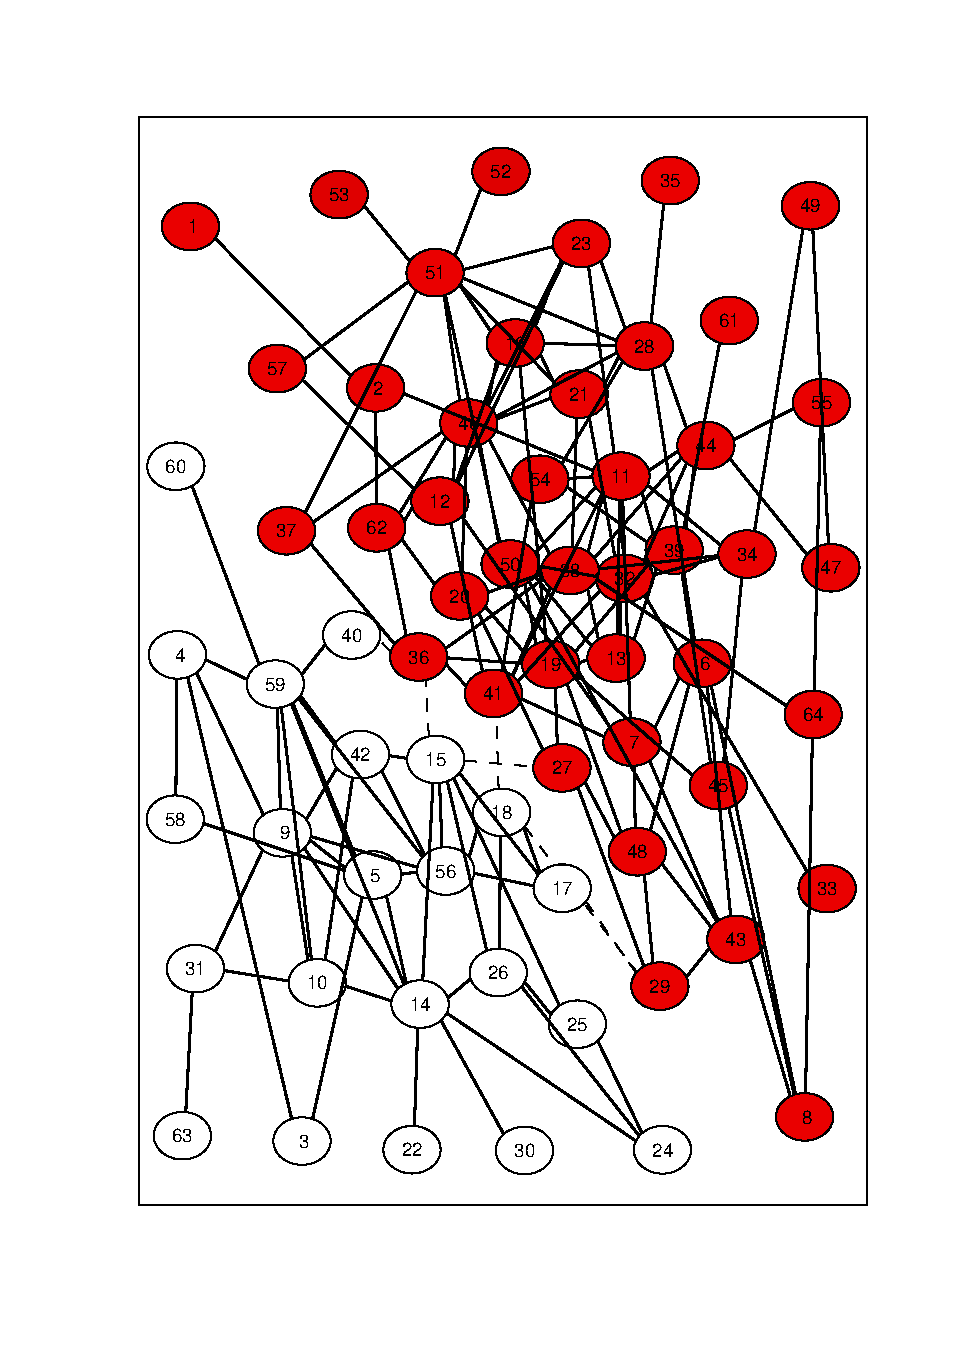
\includegraphics[width=0.6\textwidth]{do-m2-2}
		\vspace{-1cm}
		\\
		(a) (b) (c)
		\end{tabular}
	\end{center}
\end{frame}

\begin{frame}{Conclusion}
	\begin{itemize}
		\item Modèle non normalisé peu fiable, de même que l'analyse spectrale sur plus grand écart (analyse trop simpliste ?).
		\item Modèle normalisé plutôt satifsaisant, on retrouve les observations. Idem pour la séparation en 0.
		\item Il existe des méthodes plus performantes, utilisant des notions plus complexes pour les graphes (<<~modularité~>>).
	\end{itemize}
\end{frame}


\end{document}
